\begin{figure}[t]
\vspace{-6pt}
  \centering
  \includegraphics[width=0.99\textwidth]{figs/fig6.pdf}
  \vspace{-3pt}
    \captionof{figure}{\textbf{Examples of report generation and VQA from various MLLMs}. The highlighted text reflects the unique features of each image. For comparison, each image displays its modality, plane, and abnormality information at the top. Top: an example of report generation; Bottom: an example of VQA.}
    \label{fig6}
    \vspace{-6pt}
\end{figure}

  
\begin{table}[t]
  \vspace{-6pt}
  \centering
  \caption{\textbf{Performance on image-to-text tasks}. Top: Report generation performance evaluated across four datasets. Higher scores on the ROUGE, METEOR, and BERT-F1 metrics indicate better performance. Bottom: VQA performance on four datasets. "Mod." represents modality and "Abno." represents abnormality, with each value representing accuracy. \textbf{Bold} denotes the best performance, and * indicates a significant difference between ours and baselines ($p$-value$\ < 0.05$).}
  \label{table1}
  \vspace{3pt}
  \setlength{\tabcolsep}{2pt} 
  \centering
  \scalebox{0.725}{
    \centering
    \begin{tabular}{l|ccc|ccc|ccc|ccc}
        \toprule
        \multirow{2}{*}{Report Generation} &  \multicolumn{3}{c|}{BraTS2021}  & \multicolumn{3}{c|}{BraTS2023-MEN}  &  \multicolumn{3}{c|}{ATLAS 2.0} & \multicolumn{3}{c}{IXI}  \\
         & \small R. & \small M. & \small B. & \small R. & \small M. & \small B. & \small R. & \small M. & \small B. & \small R. & \small M. & \small B. \\
        \cmidrule(lr){1-13}
        \small LLaVA-Med                                 &  7.19  \ & 12.37 \ & 85.52 \ &  6.26 \ & 11.38 \ & 85.43 \ &  7.15 \ & 14.37 \ & 86.74 \ &  9.25 \ & 19.70 \ & 87.69 \ \\
        \small LLaVA 1.6                                 & 20.66  \ & 19.98 \ & 84.24 \ & 21.48 \ & 21.10 \ & 84.34 \ & 25.05 \ & 26.00 \ & 86.40 \ & 28.56 \ & 30.59 \ & 87.80 \ \\
        \small LLama 3.2 11B                             & 15.78  \ & 15.32 \ & 83.10 \ & 16.43 \ & 16.52 \ & 83.15 \ & 16.62 \ & 15.20 \ & 83.07 \ & 17.12 \ & 16.04 \ & 83.32 \ \\
        \small Gemini 1.5 8B                       & 22.04  \ & 17.69 \ & 81.94 \ & 22.01 \ & 17.28 \ & 81.67 \ & 21.63 \ & 17.66 \ & 81.90 \ & 22.65 \ & 18.30 \ & 82.06 \ \\
        \small GPT 4o-mini                               & 17.42  \ & 15.86 \ & 81.55 \ & 16.13 \ & 14.99 \ & 81.39 \ & 18.97 \ & 18.23 \ & 82.02 \ & 22.28 \ & 20.27 \ & 82.73 \ \\
        \rowcolor{gray!10} \small \textbf{LLaBIT (Ours)} & \textbf{35.03}$^*$ & \textbf{39.35}$^*$ & \textbf{89.71}$^*$ & \textbf{33.36}$^*$ & \textbf{36.84}$^*$ & \textbf{89.12}$^*$ & \textbf{33.69}$^*$ & \textbf{36.97}$^*$ & \textbf{89.44}$^*$ & \textbf{37.33}$^*$ & \textbf{41.82}$^*$ & \textbf{90.50}$^*$ \\
        \bottomrule
        \toprule
        \multirow{2}{*}{VQA} &  \multicolumn{3}{c|}{BraTS2021}  & \multicolumn{3}{c|}{BraTS2023-MEN}  &  \multicolumn{3}{c|}{ATLAS 2.0} & \multicolumn{3}{c}{IXI}  \\
         & Mo. & Pl. & Ab. & Mo. & Pl. & Ab. & Mo. & Pl. & Ab. & Mo. & Pl. & Ab.  \\
        \midrule
        \small LLaVA-Med                                 & 0.736 \ & 0.391 \ & 0.682 \ & 0.747 \ & 0.385 \ & 0.582 \ & 0.907 \ & 0.349 \ & 0.279 \ & 0.902 \ & 0.373 \ & 0.216 \ \\
        \small LLaVA 1.6                                 & 0.291 \ & 0.336 \ & 0.536 \ & 0.286 \ & 0.308 \ & 0.286 \ & 0.605 \ & 0.256 \ & 0.186 \ & 0.431 \ & 0.392 \ & 0.745 \ \\
        \small LLama 3.2 11B                             & 0.864 \ & 0.922 \ & 0.800 \ & 0.846 \ & 0.923 \ & 0.780 \ & 0.907 \ & 0.744 \ & 0.674 \ & 0.863 \ & 0.902 \ & 0.922 \ \\
        \small Gemini 1.5 8B                       & 0.664 \ & 0.745 \ & 0.500 \ & 0.670 \ & 0.681 \ & 0.549 \ & 0.767 \ & 0.791 \ & 0.605 \ & 0.745 \ & 0.804 \ & 0.902 \ \\
        \small GPT 4o-mini                               & 0.482 \ & 0.518 \ & 0.182 \ & 0.527 \ & 0.560 \ & 0.154 \ & 0.744 \ & 0.907 \ & 0.186 \ & 0.549 \ & 0.922 \ & 0.608 \ \\
        \rowcolor{gray!10} \small \textbf{LLaBIT (Ours)} & \textbf{0.945}$^*$ & \textbf{0.927}$^*$ & \textbf{0.891}$^*$ & \textbf{0.945}$^*$ & \textbf{0.945}$^*$ & \textbf{0.934}$^*$ & \textbf{0.977}$^*$ & \textbf{0.953}$^*$ & \textbf{0.721}$^*$ & \textbf{0.922}$^*$ & \textbf{0.961}$^*$ & \textbf{0.980}$^*$ \\
        \bottomrule
    \end{tabular}
    }
    \vspace{-6pt}
\end{table}
  
\begin{table}[t]
    \vspace{-6pt}
    \centering
    \caption{\textbf{Performance on image-to-image tasks}. "WT." denotes whole tumor, "ET." denotes enhancing tumor, "TC." denotes tumor core, and "Avg." represents the average value. Each value is expressed as a dice coefficient. \textbf{Bold} indicates the best performance, \underline{underlined} denotes the second best performance, and * significant difference between ours and baselines, $p$-value$\ < 0.05$.}
    \label{table2}
    \vspace{3pt}
  
  \begin{minipage}{1\linewidth}
    \setlength{\tabcolsep}{1.8pt} 
    \centering
    \scalebox{0.65}{
        \begin{tabular}{l|cccc|cccc|cccc|c}
            \toprule
            \multirow{2}{*}{Image Segmentation} &  \multicolumn{4}{c|}{BraTS2021}  & \multicolumn{4}{c|}{BraTS2023-MEN} & \multicolumn{4}{c|}{UPENN-GBM} & ATLAS 2.0\\
             & WT. & ET. & TC. & Avg. & WT. & ET. & TC. & Avg. &  WT. & ET. & TC. & Avg. & \fs \textbf{Stroke}\\
            \cmidrule(lr){1-14}
            M3D (Pretrained)              & 0.025 \  & 0.024 \  & 0.010 \  & 0.019 \  & 0.013 \  & 0.008 \  & 0.008 \  & 0.010 \  & 0.041 \  & 0.035 \ & 0.016  \ & 0.030  \ & 0.010 \  \\
            M3D (Fine-tuned)              & 0.608 \  & 0.450 \  & 0.342 \  & 0.466 \  & 0.275 \  & 0.231 \  & 0.101 \  & 0.202 \  & 0.619 \  & 0.411 \  & 0.322 \  & 0.450 \  & 0.057 \  \\
            \rowcolor{gray!10} \textbf{LLaBIT (Stage I)}    & 0.653 \  & 0.445 \  & 0.389 \  & 0.495 \  & 0.492 \  & 0.373 \  & 0.235 \  & 0.366 \  & 0.645 \  & 0.439 \  & 0.318 \  & 0.467 \  & 0.269 \  \\
            \rowcolor{gray!10} \textbf{LLaBIT (Stage II)}    & \textbf{0.770}$^*$ & \textbf{0.747}$^*$ & \textbf{0.603}$^*$ & \textbf{0.706}$^*$ & \textbf{0.651}$^*$ & \textbf{0.587}$^*$ & \textbf{0.402}$^*$ & \textbf{0.546}$^*$ & \textbf{0.792}$^*$ & \textbf{0.778}$^*$ & \textbf{0.613}$^*$ & \textbf{0.727}$^*$ & \textbf{0.438}$^*$ \\
            \bottomrule
        \end{tabular}
    } 
    \end{minipage}
    
    \vspace{1pt}
    
    \setlength{\tabcolsep}{3.2pt} 
    \centering
    \scalebox{0.65}{
        \begin{tabular}{l|ccc|ccc|ccc|ccc}
            \toprule
            \multirow{2}{*}{T1 $\rightarrow$ T2} &  \multicolumn{3}{c|}{BraTS2021}  & \multicolumn{3}{c|}{BraTS2023-MEN} & \multicolumn{3}{c|}{IXI} & \multicolumn{3}{c}{UPENN-GBM} \\
             & \fs PSNR $\uparrow$ & \fs SSIM $\uparrow$ & \fs FID $\downarrow$ & \fs PSNR $\uparrow$ & \fs SSIM $\uparrow$ & \fs FID $\downarrow$ & \fs PSNR $\uparrow$ & \fs SSIM $\uparrow$ & \fs FID $\downarrow$ & \fs PSNR $\uparrow$ & \fs SSIM $\uparrow$ & \fs FID $\downarrow$ \\
            \cmidrule(lr){1-13}
            DiffuseIT                                    & \underline{22.61} & \textbf{0.817}    & \underline{38.42} & 23.40 \              & 0.838             & 44.37             & \underline{22.93} \ & \underline{0.746} \ & 30.09 \             & 21.22 \             & \underline{0.783} \ & 49.76 \             \\
            ControlNet                                   & 22.16             & 0.810             & \textbf{32.35}    & \underline{23.57} \  & \underline{0.845} & \textbf{41.82}    & 22.64 \             & 0.712 \             & \underline{26.13} \ & \underline{22.19} \ & 0.781 \             & \underline{44.20} \ \\
            \rowcolor{gray!10} \textbf{LLaBIT (Stage I)} & 21.23             & 0.722             & 47.99             & 22.42 \              & 0.765             & 51.80             & 21.55 \             & 0.648 \             & 27.54 \             & 21.02 \             & 0.707 \             & 45.38 \             \\
            \rowcolor{gray!10} \textbf{LLaBIT (Stage II)} & \textbf{22.99}    & \underline{0.815} & 42.83             & \textbf{24.32}$^*$   & \textbf{0.846}    & \underline{43.56} & \textbf{23.93}$^*$  & \textbf{0.793}$^*$  & \textbf{24.82}$^*$  & \textbf{22.94}$^*$  & \textbf{0.817}$^*$  & \textbf{43.20}$^*$  \\
            \bottomrule
        \end{tabular}
    }
    \centering
    \vspace{-6pt}
\end{table}



\section{Results}
\noindent \textbf{Report Generation.} We compared the report generation performance of our model with that of other vision-language models that accept images as input along with instructions. The results show that our model achieved the best scores on the ROUGE, METEOR, and BERT-F1 metrics (Table \ref{table1} top). Fig. \ref{fig6} left shows representative outputs from each model. While the reports from the other models contain unnecessary or inaccurate information and lack detailed image descriptions, our model captures all the essential information. This suggests that instruction tuning of the language model with our data generation better captures rich image details. Note that this evaluation is inherently limited, as it relies on LLM-generated data instead of clinician-written reports. Nevertheless, the primary objective of this study was not to produce a flawless clinical report generator, but to demonstrate that a single fine-tuned LLM can be proficient in both image-to-image and image-to-text tasks.

\vspace{3pt}
\noindent \textbf{Visual Question Answering.} We evaluated the VQA performance of our model and other models using three question types to measure image understanding. The questions focus on modality, plane, and abnormality. They are posed in a closed-ended format to ensure that the models provide definite answers. An example of these VQA results is shown in Fig. \ref{fig6} right. We measured answer accuracy of correct answers across four datasets and three question types. The results for each model are summarized in Table \ref{table1} bottom. Our model outperformed other models on every metric, demonstrating an enhanced understanding of brain MR images in terms of modality, plane, and abnormality. 

\vspace{3pt}
\noindent \textbf{Segmentation.} We compared the segmentation performance of our method with M3D, a language model that can perform segmentation (Table \ref{table2} top). Unlike M3D, which relies on an additional segmentation module (such as SegVol \cite{du2024segvol}), our approach uses a single transformer that generates segmentation tokens autoregressively. 
Since the pretrained M3D, which has been trained on various medical datasets, has not seen brain MR images, its performance suffers in brain tumor segmentation. For a fair comparison, we also fine-tuned M3D on the same training dataset as ours. The segmentation results, as shown in Fig. \ref{fig7}, indicate that while the segmentation tokens generated in Stage I are able to roughly segment the lesion area, the Stage II module adds much more detail.

\vspace{3pt}
\noindent \textbf{Image Translation.} Since no previous study has addressed image translation using a language model, we trained and compared models that use text encoders, such as those from CLIP encoders pretrained via contrastive learning on image data, on the same image-text paired dataset. Quantitative results are shown in Table \ref{table2} bottom and qualitative results are shown in Fig. \ref{fig8}. Although it is challenging to outperform models specifically designed for image synthesis with strong inductive bias, our method achieved competitive performance. Furthermore, skip connections led to a noticeable improvement, suggesting that they help to capture fine details more effectively.


\begin{figure} [t]
    \centering
    \begin{minipage}{0.48\columnwidth}
        \centering
        \includegraphics[width=\columnwidth]{figs/fig7.pdf}
        \vspace{-6pt}
        \caption{\textbf{Segmentation results}. Top:  BraTS-2021. Bottom: ATLAS 2.0.}
        \label{fig7}
        \end{minipage}
        \begin{minipage} {0.08\textwidth}
        \end{minipage}
        \begin{minipage}{0.48\columnwidth}
        \centering
        
\includegraphics[width=\columnwidth]{figs/fig8.pdf}
        \vspace{-6pt}
        \caption{\textbf{T1 $\rightarrow$ T2 translation results.} Top: UPENN-GBM. Bottom: IXI.}
        \label{fig8}
    \end{minipage}
\end{figure}

\begin{table} [t]
    \centering
    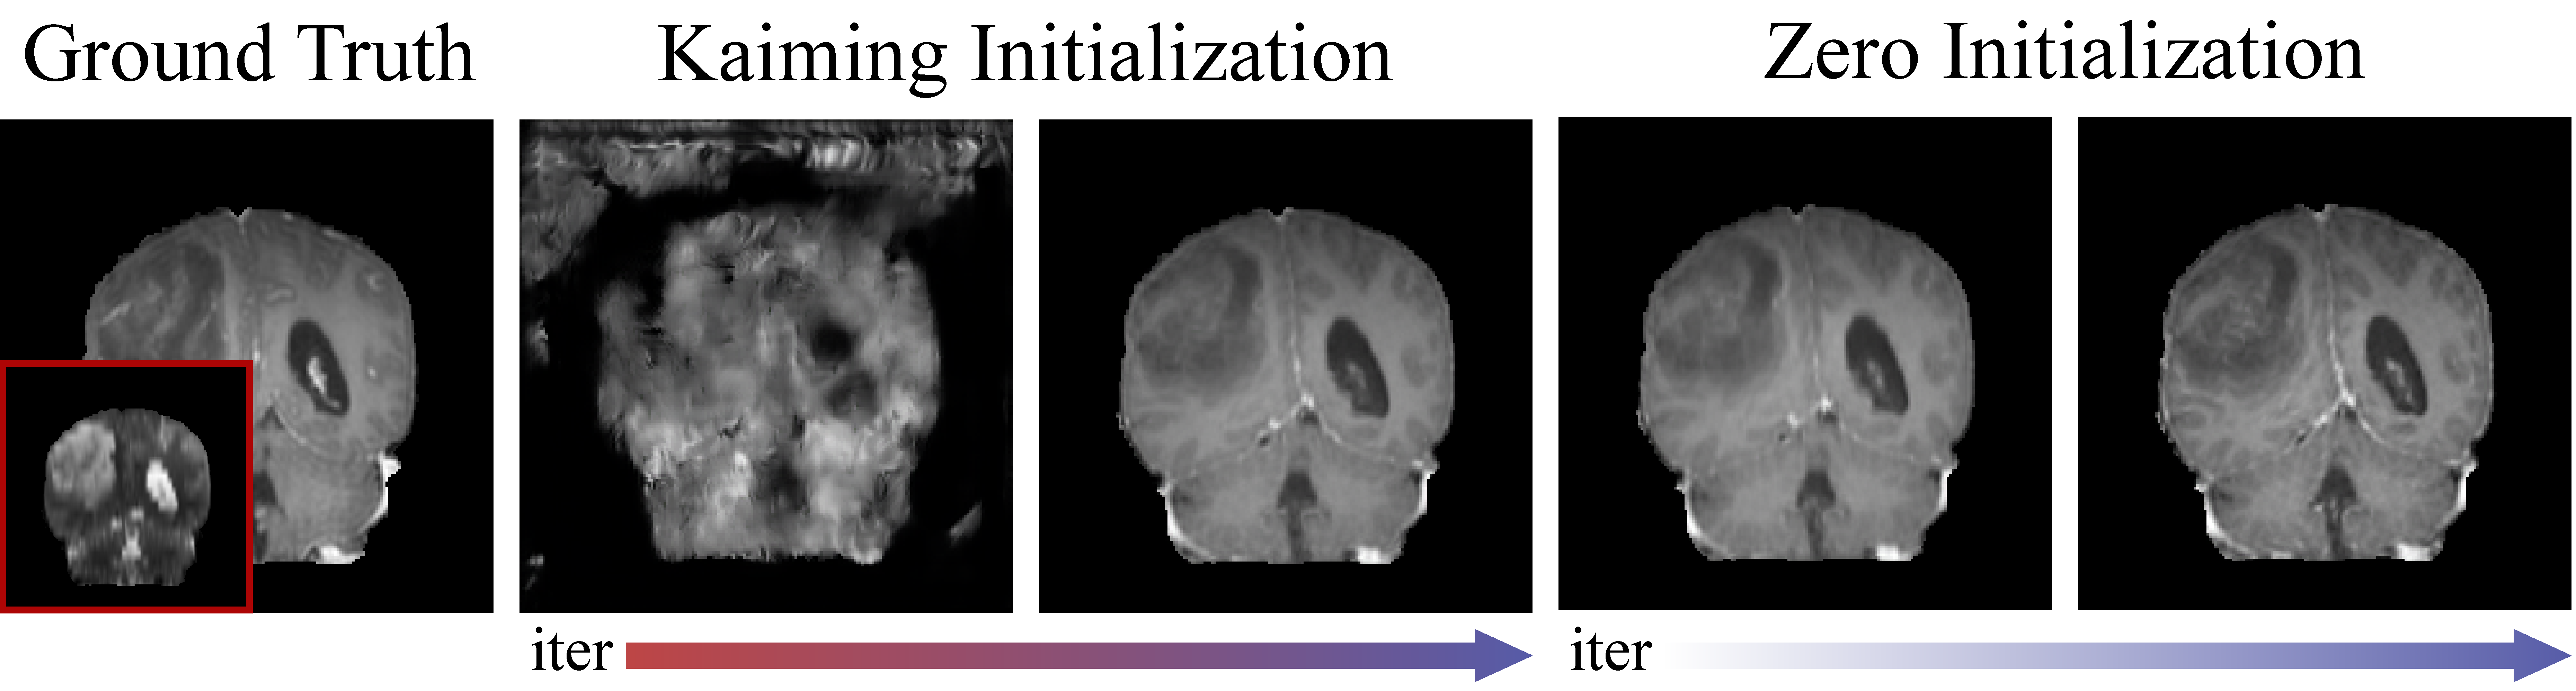
\includegraphics[width=0.65\columnwidth]{figs/fig9.pdf}
    \vspace{3pt}
    \captionof{figure}{\textbf{Comparison of two initialization methods in the skip connection block for T2 $\rightarrow$ T1ce translation.} With Kaiming initialization, the image degrades rapidly early on. Zero initialization leads to a gradual increase in detail.}
    \label{fig9}
    \centering
    \captionof{table}{\textbf{Evaluation of generated report and VQA data}. GPT 4o is used to score the outputs on a scale from 0 to 10 based on predefined criteria.}
    \label{table3}
    \setlength{\tabcolsep}{12pt} 
    \centering
    \scalebox{0.75}{
        \begin{tabular}{l|cc}
            \toprule
            Model & Report generation & VQA generation \\
            \cmidrule(lr){1-3}
            Gemini 1.5 8B & 6.275 \small $\pm$ 2.667 & 8.008 \small $\pm$ 2.351 \\
            LLaMA 3.2 11B & 5.189 \small $\pm$ 1.799 & 6.837 \small $\pm$ 1.848 \\
            GPT 4o-mini  & 7.232 \small $\pm$ 2.106 & 8.025 \small $\pm$ 1.284 \\
            \midrule
            \textbf{Refined Data}  & \textbf{7.939 \small $\pm$ 2.174} & \textbf{8.538 \small $\pm$ 0.875} \\
            \bottomrule
        \end{tabular}
    }
    \centering
    \vspace{-6pt}
\end{table}

\vspace{3pt}
\noindent \textbf{Text Data Generation with LLMs.} We evaluated text data generated by our instruction-driven pipeline, which was designed to produce text data for image-only datasets. In this evaluation, we provided our generated text and evaluation criteria (from BioMed-VITAL \cite{cui2024biomedical}) to GPT 4o \cite{achiam2023gpt}, which scored the outputs on a scale from 0 to 10. Table \ref{table3} shows the average scores for generated reports and VQA outputs across different models. Among the individual language models, GPT 4o-mini achieved the highest score. When outputs from all three models were combined, the average score improved. 

\vspace{3pt}
\noindent \textbf{Ablation Study.} We performed an ablation study on each component of our method for image translation tasks with the results shown in Table \ref{table4}. Although using only the autoregressively generated image tokens from Stage I is sufficient for image-to-image synthesis, adding a learnable convolutional block significantly improved performance. In addition, zero initialization allowed the model to learn gradually, and both BiomedCLIP \cite{zhang2023biomedclip} and prompt tuning helped improve performance by allowing the model to adapt its features according to the target.

\begin{table} [t]
    \vspace{-6pt}
    \caption{\textbf{Ablation study results on the UPENN-GBM}. }
    \label{table4}
    \vspace{3pt}
    \setlength{\tabcolsep}{8pt} 
    \centering
    \scalebox{0.725}{
        \begin{tabular}{l|cccc|cccc}
            \toprule
            & \multicolumn{4}{c}{Segmentation} & \multicolumn{4}{|c}{T1 $\rightarrow$ T2} \\
              & WT. & ET. & TC. & Avg. & PSNR $\uparrow$ & SSIM $\uparrow$ & FID $\downarrow$ & LPIPS $\downarrow$  \\
            \cmidrule(lr){1-9}
            Stage I only      & 0.645 & 0.439 & 0.318 & 0.467 & 21.023 & 0.707 & 45.382 & 0.146 \\
            + Skip Conv block & 0.705 & 0.617 & 0.515 & 0.612 & 21.811 & 0.757 & 48.018 & 0.138 \\
            + Zero init       & 0.725 & 0.653 & 0.534 & 0.637 & 22.312 & 0.778 & 45.723 & 0.124 \\
            + Prompt tuning   & 0.773 & 0.762 & 0.608 & 0.714 & 22.617 & 0.801 & 45.047 & 0.117 \\
            + BioMedCLIP      & \textbf{0.792} & \textbf{0.778} & \textbf{0.613} & \textbf{0.727} & \textbf{22.943} & \textbf{0.817} & \textbf{43.205} & \textbf{0.111} \\
            \bottomrule
        \end{tabular}
    }
    \vspace{-6pt}
\end{table}

% \noindent \textbf{Nucleus Sampling.} 

\vspace{3pt}
\noindent \textbf{Impact of Zero Initialization.} We compared how different parameter initializations affect the training of the skip connection block. Fig. \ref{fig9} shows the comparison between the Kaiming initialization \cite{he2015delving} and the zero initialization. When Stage II starts with non-zero initial values, these early values tend to dominate, whereas zero initialization allows the model to gradually update its parameters while preserving the image features learned from the Stage I tokens. This approach not only improves performance but leads to more stable training.
